%!TEX root = ../main.tex

Nesta seção serão apresentados os resultados parciais obtidos no treinamento de modelos baseados em algumas das arquiteturas selecionadas para o escopo deste trabalho. \todo{Terminar a apresentação das seções após o término da análise dos modelos treinados}


\subsection{Resultados Obtidos com a CNN LeNet}
\label{sec:lenet}

A primeira fase do treinamento dos modelos foi dada utilizando a arquitetura LeNet. Nesta fase, foi realizada uma busca em \emph{grid} por todos os hiperparâmetros previamente definidos, gerando um total de 108 modelos no total. Alguns desses modelos tiveram seus resultados degenerados, ou seja, não conseguiram aprender e acabaram voltando suas saídas para apenas um valor.

Considerando a métrica de \emph{F-score} como referência, foi possível identificar os melhores resultados utilizando conjunto de testes de cada uma das três abordagens conforme a Tabela \ref{tab:lenet}.

\begin{table}[h!]
\centering
\caption{Detalhamento dos melhores modelos obtidos com a arquitetura LeNet, organizados de forma descrescente considerando o valor de Acurácia.}
\label{tab:lenet}
\begin{tabular}{cccccc}
\toprule
\textbf{Conjunto} & \textbf{Otimizador} & \textbf{\emph{Patience}}  & \textbf{Função de Ativação} & \textbf{Acurácia} & \textbf{F-Score} \\
\midrule
Abordagem 1 & RMSprop & 5 & SELU & $0.7224$ & $0.1794$ \\
Abordagem 2 & Adam & 5 & ReLU & $0.5088$ & $0.6036$ \\
Abordagem 3 & RMSprop & 5 & ELU & $0.4696$ & $0.5099$ \\
\bottomrule
\end{tabular}
\end{table}

Os gráficos da Figura \ref{fig:treinamento-lenet} denotam o histórico da perda (\emph{loss}) e acurácia para o conjunto de treinamento e validação destas redes. Nota-se que nenhuma delas chegou ao limite máximo de épocas possíveis, interrompendo o aprendizado por meio de \emph{early stopping}.


\begin{figure}[h!]
	\centering
	\caption{Histórico de \emph{loss} e acurácia durante o treinamento dos melhores modelos obtidos com a arquitetura LeNet.}
	\subfloat[Abordagem 1 com RMSprop, SELU e \emph{patience} igual a 5\label{subfig:approach1-lenet}]{%
	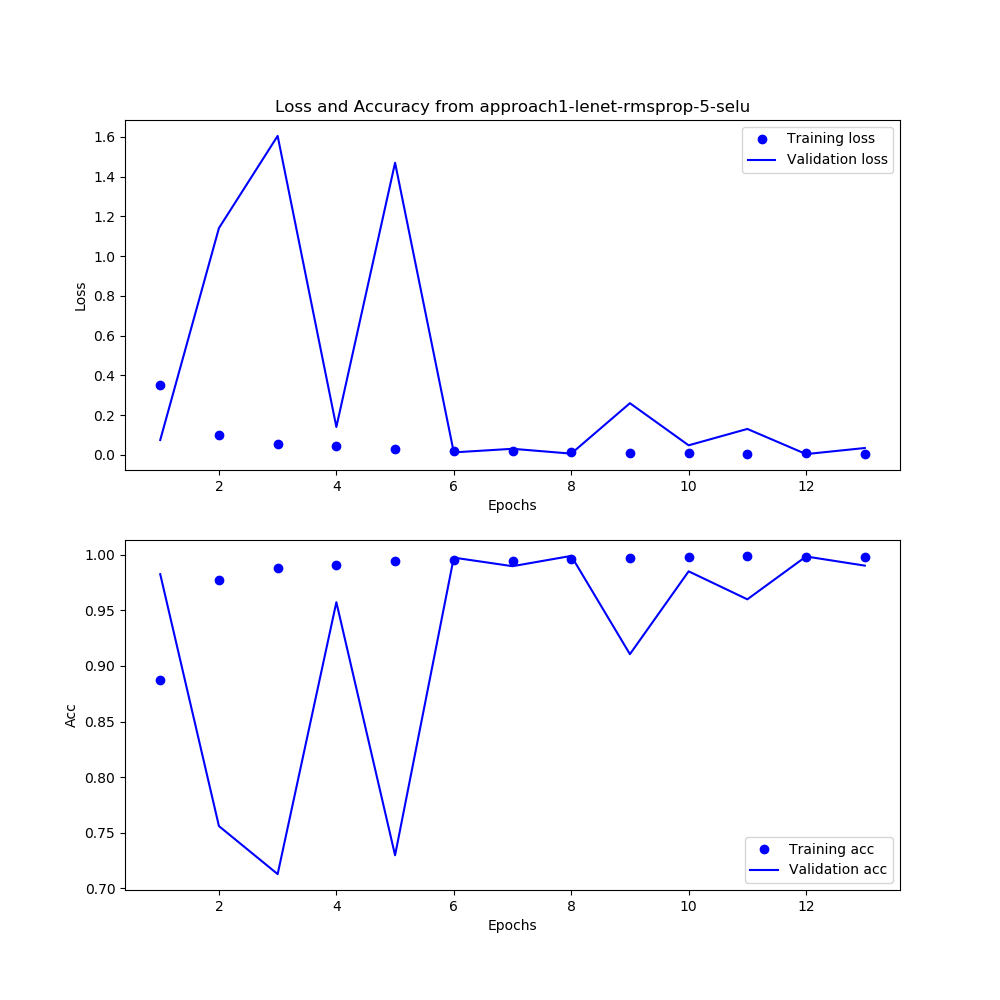
\includegraphics[width=0.5\textwidth]{imgs/approach1-lenet-rmsprop-5-selu}
	}
	\subfloat[Abordagem 2 com Adam, ReLU e \emph{patience} igual a 5\label{subfig:approach2-lenet}]{%
	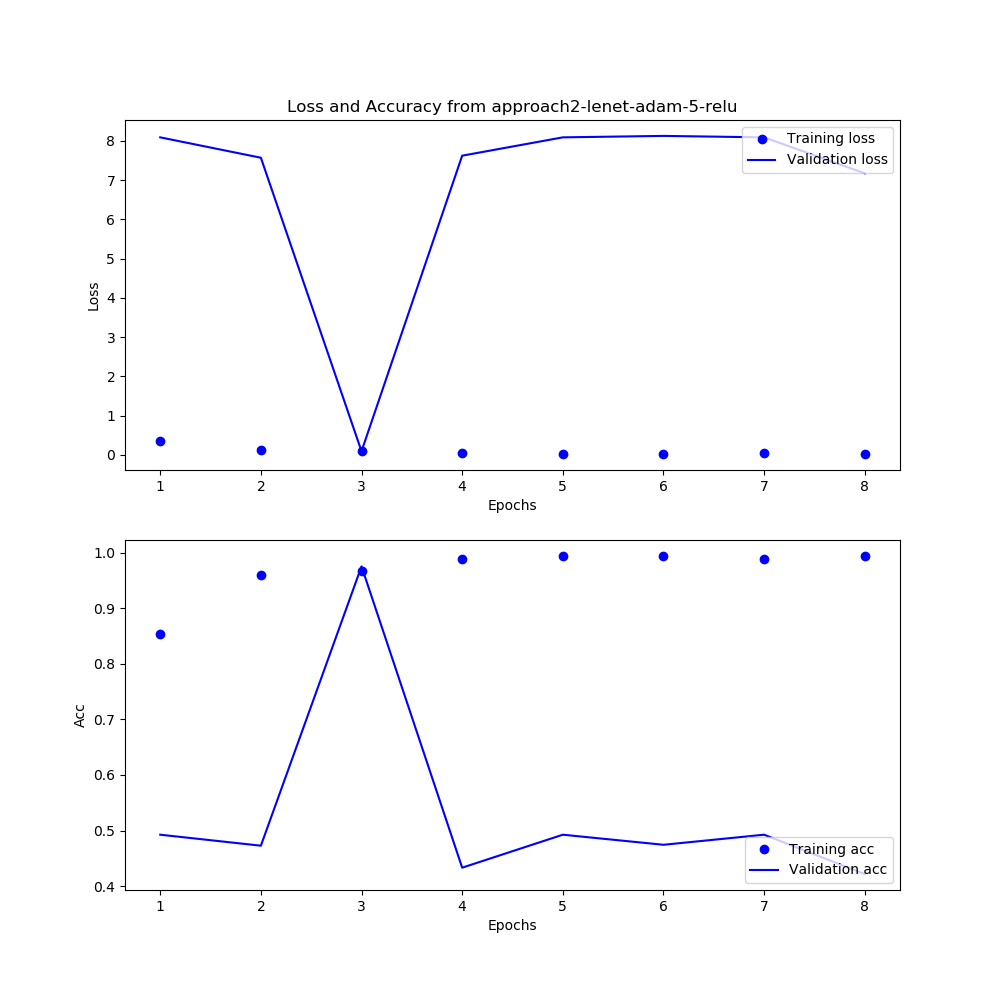
\includegraphics[width=0.5\textwidth]{imgs/approach2-lenet-adam-5-relu}
	}
	\hfill
	\subfloat[Abordagem 3 com RMSprop, ELU e \emph{patience} igual a 5\label{subfig:approach3-lenet}]{%
	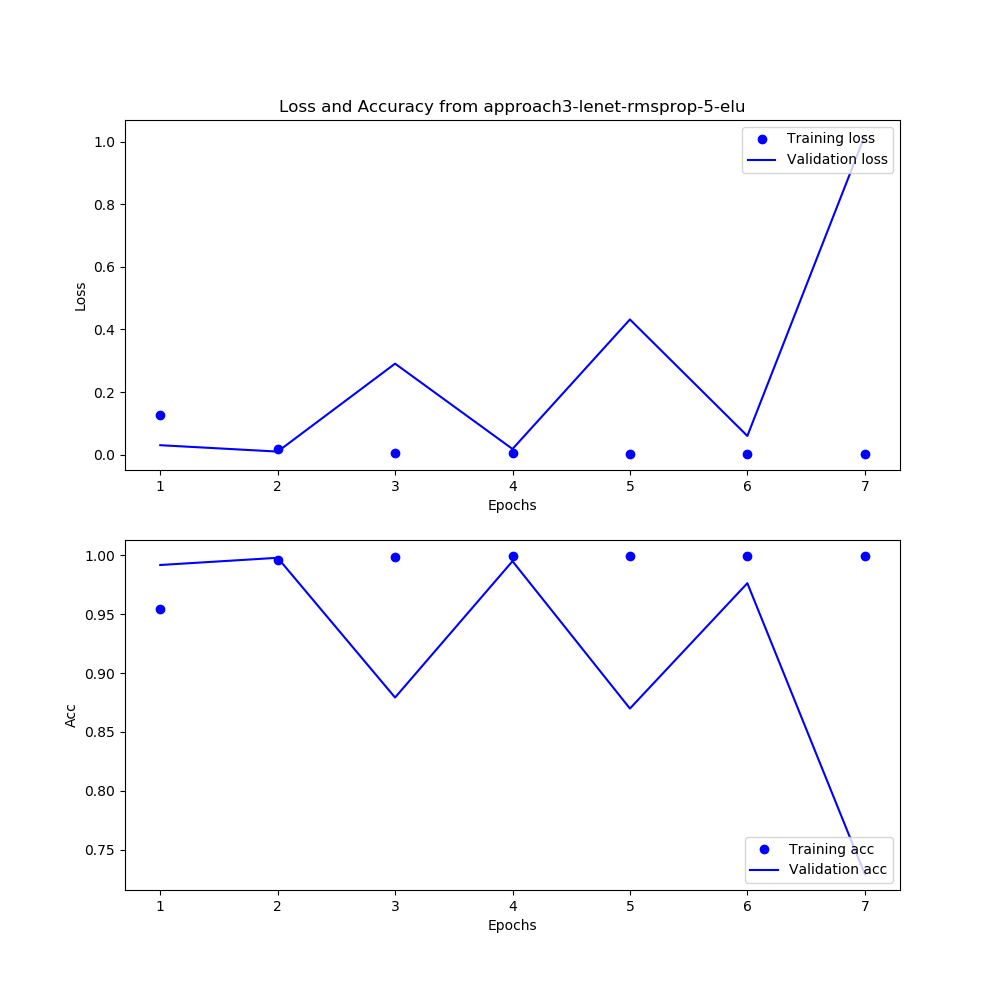
\includegraphics[width=0.5\textwidth]{imgs/approach3-lenet-rmsprop-5-elu}
	}
	\label{fig:treinamento-lenet}
\end{figure}

Examinando mais atentamente o desempenho destas redes, tem-se, então, as matrizes de confusão mostradas na Figura \ref{fig:matrizes-lenet}. Nestas matrizes, a soma das linhas representam a quantidade de assinaturas previstas para cada classe pelo modelo em questão, enquanto a soma das colunas denotam a quantidade de assinaturas existentes em cada classe.

\begin{figure}[h!]
	\centering
	\caption{Matrizes de confusão dos melhores modelos obtidos com a arquitetura LeNet.}
	\subfloat[Abordagem 1\label{subfig:matriz-approach1-lenet}]{%
	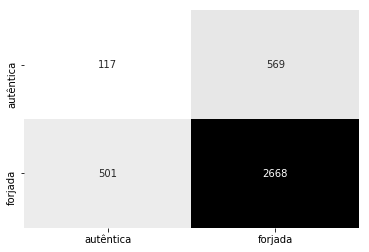
\includegraphics[width=0.5\textwidth]{imgs/matriz-approach1-lenet}
	}
	\subfloat[Abordagem 2\label{subfig:matriz-approach2-lenet}]{%
	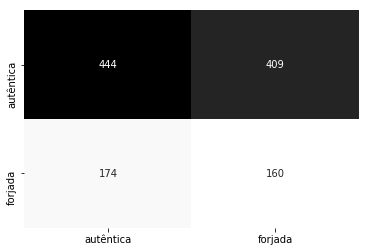
\includegraphics[width=0.5\textwidth]{imgs/matriz-approach2-lenet}
	}
	\hfill
	\subfloat[Abordagem 3\label{subfig:matriz-approach1-lenet}]{%
	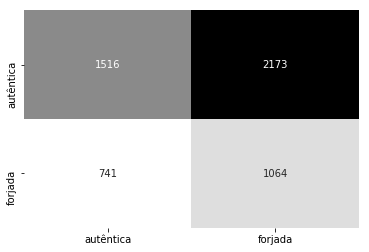
\includegraphics[width=0.5\textwidth]{imgs/matriz-approach3-lenet}
	}
	\label{fig:matrizes-lenet}
\end{figure}

%%%% ARGUMENTAÇÃO

Para esta arquitetura, é possível visualizar que, os melhores modelos foram aqueles que possuiam o menor valor de \emph{patience}. Isso demonstra que foi necessário poucas épocas de treinamento para obter modelos melhores que a maioria. É importante afirmar também que, mesmo com a mudança de hiperparâmetros, as métricas de desempenho resultantes de modelos que foram treinados perante uma mesma abordagem não obtiveram uma grande variação. Isso demonstra que o balanceamento dos conjuntos de dados, no caso desta topologia, foi essencial para a obtenção de melhores resultados.



\subsection{Resultados Obtidos com a CNN AlexNet}
\label{sec:alexnet}
 %% Trabalhar aqui

 Para a AlexNet, assim como para a CNN anterior, foi realizada uma busca em \emph{grid} com os hiperparâmetros selecionados anteriormente, com vistas a obter os melhores modelos para cada abordagem de separação de dados, gerando assim, mais 108 modelos a serem avaliados quanto as suas métricas de desempenho.

 Mais uma vez considerando a métrica de \emph{F-score}, foram selecionados os melhores modelos e estes encontram-se listados na Tabela \ref{tab:alexnet}.

 \begin{table}[h!]
 \centering
 \caption{Detalhamento dos melhores modelos obtidos com a arquitetura AlexNet, organizados de forma descrescente considerando o valor de Acurácia.}
 \label{tab:alexnet}
 \begin{tabular}{cccccc}
 \toprule
 \textbf{Conjunto} & \textbf{Otimizador} & \textbf{\emph{Patience}}  & \textbf{Função de Ativação} & \textbf{Acurácia} & \textbf{F-Score} \\
 \midrule
 Abordagem 3 & Adam & 15 & SELU & $0.4456$ & $0.5524$ \\
 Abordagem 2 & SGD & 5 & \emph{Leaky} ReLU & $0.5282$ & $0.6349$ \\
 Abordagem 1 & RMSprop & 5 & ReLU & $0.1844$ & $0.2765$ \\
 \bottomrule
 \end{tabular}
\end{table}


\begin{figure}[h!]
	\centering
	\caption{Matrizes de confusão dos melhores modelos obtidos com a arquitetura AlexNet.}
	\subfloat[Abordagem 1\label{subfig:matriz-approach1-alexnet}]{%
	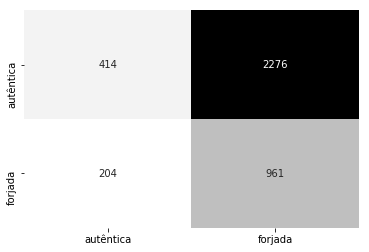
\includegraphics[width=0.5\textwidth]{imgs/matriz-approach1-alexnet}
	}
	\subfloat[Abordagem 2\label{subfig:matriz-approach2-alexnet}]{%
	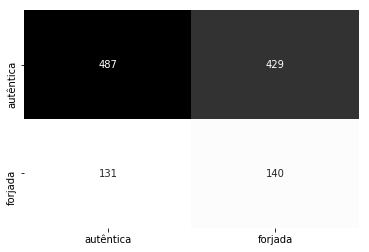
\includegraphics[width=0.5\textwidth]{imgs/matriz-approach2-alexnet}
	}
	\hfill
	\subfloat[Abordagem 3\label{subfig:matriz-approach1-alexnet}]{%
	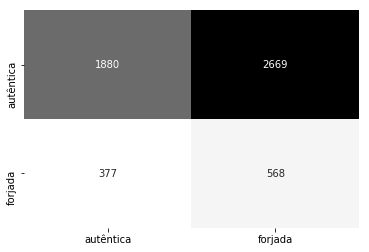
\includegraphics[width=0.5\textwidth]{imgs/matriz-approach3-alexnet}
	}
	\label{fig:matrizes-alexnet}
\end{figure}

\subsection{Resultados Obtidos com a CNN SqueezeNet}
\label{sec:squeezenet}

\subsection{Resultados Obtidos com a CNN MobileNet}
\label{sec:mobilenet}
